\chapter{Diseño del solver y compilador}\label{chapter:dise_solver_compilador}

En este capítulo se explicará el funcionamiento del proceso
de compilación del lenguaje así como varios conceptos importantes relacionados.
Este proceso de compilación es también un proceso de resolución de problemas y
es el responsable de conseguir las soluciones a las entradas proporcionadas.

%------------------------- Árbol Sintáctico Abstracto ------------------------%
\section{Árbol Sintáctico Abstracto}
La estructura obtenida del \textit{Parser} que contiene toda la información posible es 
el Árbol Sintáctico Abstracto. En este se encuentran tanto las definiciones de 
variables como las restricciones. Contiene también la estructura principal, 
las auxiliares y las funciones, sean estas o no utilizadas.

No hubo necesidad de generar una tabla de símbolos ya que a diferencia de 
otros lenguajes los valores de las variables solo pueden pasar de no asignado a 
asignado y luego no hay posibles modificaciones. De hecho solo si la variable es 
constante su valor comienza siendo asignado, de resto no será sino hasta los últimos 
pasos del proceso de compilación cuando consiga un valor concreto.

El árbol luce como la figura \ref{fig:ast} y contiene:

\begin{itemize}
 \item {Las estructuras de la representación.}
 \item {La descripción de las variables así como sus posibles restricciones 
	individuales y globales.}
 \item {Las funciones particulares que el usuario describió.}
\end{itemize}

\begin{figure}[h]
	\begin{center}
		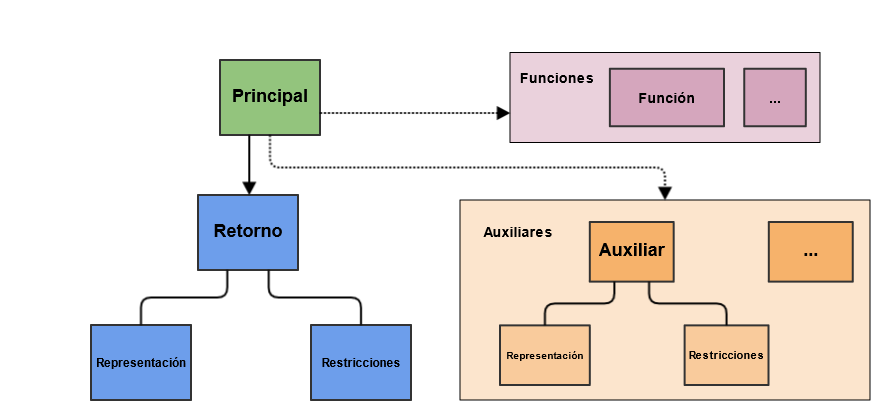
\includegraphics[scale=0.55]{imagenes/AST.png}
	\end{center}
	\caption{
		\label{fig:ast}
		Gráfica del AST
	}
\end{figure}

%------------------ Grafo y generación de estructura de retorno ------------------%
\section{Grafo y generación de estructura de retorno}
Dentro del compilador no será suficiente contar con el \textbf{AST} para hacer los cálculos 
necesarios y obtener las soluciones. Para estos se utilizarán dos estructuras: 
\begin{itemize}
 \item {Un grafo: Que delimitará los grupos de variables y se encargará de calcular 
	los valores de soluciones finales.}
 \item {Una estructura de salida: Que será el equivalente a la estructura 
	especificada. En esta se almacenarán los valores de las variables finales y 
	luego servirá para producir la salida en formato genérico.}
\end{itemize}


\section{Aclaraciones iniciales sobre el solver}
Antes de explicar el funcionamiento del \emph{solver} es necesario primero definir 
ciertos conceptos clave para entender su funcionamiento.

\subsection{Sistemas de variables}
\label {sis_variables}
Hay que tener claro que una parte fundamental del \emph{Solver} es como bien su nombre 
lo sugiere solucionar problemas, esto debido, a su naturaleza de 
\textbf{CSP}. Para esto hay que analizar y conseguir todos los posibles valores que se le 
pueda dar a cada variable, en especial a aquellas que dependan de otras variables.
Debido a que no todas las restricciones son de tipo algebraico se prefiere 
llamarlo \emph{sistema de variables} más que el tradicional concepto de \emph{sistema de 
ecuaciones}.

Entonces, para definir claramente un \emph{sistema de variables} hay que considerar los
siguientes puntos:

\begin{itemize}
 \item {Un conjunto de variables forman un sistema si existen restricciones que
  las involucren entre ellas de forma transitiva.}
 \item {Es posible encontrar muchos sistemas dentro de un mismo problema.}
 \item {Ya que no existen relaciones entre varios sistemas cada uno es totalmente 
  independiente de los otros y por lo tanto, el proceso de resolución que 	
  se explicará más adelante es aplicado a cada sistema independientemente.}
\end{itemize}

\subsection{Conjuntos}
Para poder representar los posibles valores que se pueden asignar a una variable
es necesario utilizar un tipo de dato o alguna notación que permita representar
conjuntos de datos. En especial grandes conjuntos ordenados de enteros.

Para esto, se ha pensado en utilizar alguna representación no expandida como 
listas por comprensión o alguna otra diseñada para este fin. Por ejemplo algo como 
esto: Los números entre -300 y 500 más los números del 550 al 600 sin incluir los
pares tendría la siguiente representación $([-300 .. 500] \cup [550..600]) - pares()$.

Sin embargo, debido a la complicación de representar los datos de esa forma en el 
lenguaje principal del \emph{Solver}, lo cual posiblemente llevaría a la implementación de 
otro sub-lenguaje, se decidió que los conjuntos de valores se representaran como 
los rangos iniciales de las variables y las listas de restricciones de dominio 
(que serán explicadas en los siguientes puntos). Cuando llegue el momento serán 
evaluadas y por ende expandidas, para ser almacenadas en archivos en memoria 
secundaria y evitar sobrecargar la memoria del programa.

\subsection{Restricciones}
Hay dos tipos de restricciones que se pueden declarar en los modelos de entrada.
Cada uno de ellos tiene sus propias implicaciones a nivel de resolución:

\subsubsection{Restricciones de dominio}
Estas son las restricciones más básicas que pueden definirse y son esenciales 
para definir el dominio de valores que pueden dársele a cada variable, 
independientemente del resto de las variables. Estas se caracterizan por lo siguiente:
\begin{itemize}
 \item {Se declaran en el área de descripción de las estructuras.}
 \item {Permiten, como su nombre lo indica delimitar los valores que 
  pueden obtener las variables sin importar el de las demás.}
 \item {Son aquellas referentes a una sola variable.}
\end{itemize}

Adicionalmente hay dos formas distintas de restricciones de dominio:

\begin{enumerate}
	\item {\textbf{Restricciones genéricas de dominio}:
Se refieren a las restricciones definidas sobre una variable básica
en alguna estructura. Estas restricciones definen el comportamiento de dicha 
variable de forma general y por lo tanto, cada instancia de la estructura que la 
contiene someterá a la variable en cuestión de la misma forma. Este tipo de 
restricción es especialmente útil para cuando se instancian muchas objetos de una 
misma estructura y se quiere que el comportamiento de sus variables sea el mismo.}

	\item {\textbf{Restricciones propias de dominio}: 
Son las restricciones que se asocian a 
una variable de tipo no básico o estructural, estas restricciones por ende hacen 
referencia a alguna de las variables básicas internas de la estructura. La 
diferencia entre este tipo de restricción con la anteriormente mencionada es que 
para estas las restricciones, sólo afectan la instancia particular asociada a la 
variable que se está restringiendo y por ende, las demás variables del mismo tipo 
no se verán afectadas. Este caso es de especial utilidad cuando existen varias 
variables de un mismo tipo de estructura, pero se quiere que cada una tenga un 
comportamiento distinto de las demás (tanto como se quiera y respetando las 
restricciones genéricas a su tipo y las restricciones de rango que se explicarán 
a continuación).}
\end{enumerate}


	
\subsubsection{Restricciones de rango}
Un problema sería muy sencillo de resolver si sus variables no se relacionaran 
entre sí. De hecho si no se relacionasen bastaría con calcular los dominios de 
cada variable y decir que esos son definitivamente los valores finales que puede 
tomar cada una. Sin embargo este tipo de problemas no es realmente un reto y por 
otro lado no permitiría definir estructuras complicadas e interesantes. Por 
ejemplo si se quisiera generar figuras humanas se quisiera que sus partes 
contaran con algo de simetría o que se rijan bajo ciertas proporciones, desde las 
más simples como las proporciones de alto y ancho hasta cosas más complicadas 
como definir que mientras más rojizo es el color del pelo más pecas podría tener 
en la cara. Incluso para cosas tan simples como calcular una distancia. es 
necesario relacionar varias variables y para esto hay que definir un tipo de 
restricción particular.

Ya que el resultado de estas restricciones condiciona directamente las posibles
respuestas finales, se ha decidido nombrarlas como \textbf{restricciones de rango}. Y estas 
restricciones cumplen con las siguientes propiedades:

\begin{itemize}
 \item {Son aquellas que relacionan algunas variables con otras.}
 \item {Se especifican en el área de restricciones.}
 \item {Permiten delimitar el rango y por lo tanto filtran el conjunto de vectores 
  de resultados posibles.}
 \item {Son realmente las únicas que presentan 	dificultad para calcularse, ya que
  dependerán de algún método de	resolución. Sea este \emph{backtracking} o métodos 
  numéricos, cosa que será tratada más adelante.}
 \item {Casi siempre cuando se hable de restricciones en 	este documento se 
  referirá a este tipo de restricciones.}
\end{itemize}

Al igual que para las restricciones de dominio, las restricciones de rango pueden 
afectar de forma genérica a un mismo tipo de estructura (restricciones genéricas 
de rango) o pueden afectar solo a una instancia particular (restricciones propias 
de rango). El razonamiento es prácticamente el mismo que ya se mencionó para las
restricciones de dominio así que se omitirá repetir esta explicación.

\subsubsection{Relación dominio-rango}
Para poder conseguir valores solución es necesario cumplir con dos condiciones: 
la primera implica que la variable en cuestión pueda tomar el valor sugerido; 
la segunda que el valor que tome la variable en conjunto con el de las demás 
cumplan con todas las restricciones de rango. Ambas condiciones son absolutamente 
necesarias o los valores no tendrían sentido dentro del problema que se quiere 
resolver. Ahora bien es importante analizar de que forma se afectan las restricciones 
de dominio y de rango entre ellas:

En primer lugar, las restricciones de dominio son propias para cada variable y por 
ende son totalmente independientes. Es decir que una restricción de dominio en 
una variable no afectará los valores posibles de otras variables y viceversa (no 
se considera el efecto de las restricciones de rango). Entonces las restricciones 
de dominio pueden calcularse todas al mismo tiempo o unas antes que otras.

Otra observación es que entre las restricciones de dominio y de rango tampoco hay 
relación, es decir que se podría decidir evaluar primero las restricciones de 
dominio y luego utilizar estos valores para y filtrar aquellos que cumplan las 
de rango; por otro lado, podría también evaluarse los de rango y conseguir los vectores solución 
para luego filtrar las soluciones viables de las que no por los valores válidos 
de dominio.

Por último, las restricciones de rango dentro de un mismo sistema de variables
deben y necesitan ser evaluadas al mismo 
tiempo siempre. 
Ahora bien, si estas restricciones no se encuentran en los mismos sistema de variables,
pueden evaluarse en cualquier orden al igual que pasaría con las 
restricciones de dominio.

\begin{itemize}
 \item {Las restricciones de dominio y las de rango son totalmente independientes 
  entre sí y solo se consideran simultáneamente a la hora de buscar el o los 
  resultados finales.}
 \item {Las restricciones de dominio pueden ser aplicadas en orden arbitrario 
  (exceptuando los casos en los que involucran funciones -no consideradas por 
  ahora-). Al ser aplicadas van acortando el conjunto de valores que puede tomar 
  la variable.}
\end{itemize}

\section{Árbol de Salida}
\label{arbol_de_salida}
Para devolver la estructura deseada ya estando inicializada hace falta primero 
construir la estructura y expandir todas sus sub-estructuras. Para esto se utiliza 
el modelo que ya se construyó en el \textbf{AST}.

Este árbol contiene variables que tomarán valores una vez se hayan resuelto todos
los sistemas de variables del problema y una vez completo se aplicará una función 
para convertir a este en un \emph{string} con formato genérico ya sea un \emph{XML} o un \emph{JSON}.
La estructura de salida será representada por un árbol y cuya estructura es similar al de la figura 
\ref{fig:estructura_salida}.

\begin{figure}[h]
	\begin{center}
		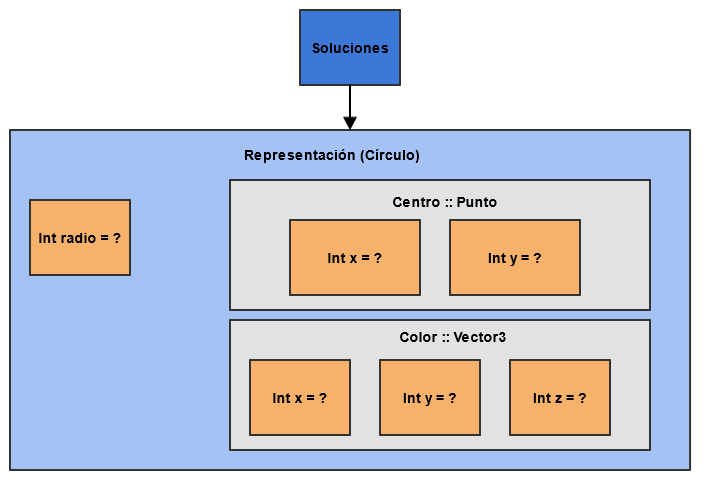
\includegraphics[scale=0.55]{imagenes/salida.png}
	\end{center}
	\caption{
		\label{fig:estructura_salida}
		Gráfico de Árbol de salida
	}
\end{figure}

\begin{itemize}
 \item {Cada elemento del árbol es o un nodo estructura (que actúa como 
  contenedor) o un tipo básico que representa una de las variables de la 
  estructura.}
 \item {Los contenedores son las expansiones de las estructuras auxiliares que 
  son contenidas por la estructura de retorno o incluso las que son contenidas 
  por otras estructuras auxiliares.}
 \item {Mientras se resuelven los sistemas las variables cuyos valores no sean 
  asignados constantes por defecto no habrán sido inicializadas.}
\end{itemize}


\section{Grafo de resolución}
Los grafos son una excelente herramienta para representar datos relacionados 
entre sí. Su forma permite realizar operaciones rápidamente y evitar
redundancias. En este caso, es necesario el uso de un grafo por la facilidad que 
ofrece para representar todas las partes de los sistemas de variables. En este
caso, el grafo del compilador se utiliza para almacenar la información necesaria con
la que se realizará el cálculo de rangos solución.

La estructuración del grafo es la siguiente: los nodos serán utilizados para almacenar 
los datos referentes a las variables, mientras que los arcos tendrán las 
restricciones de rango. De esa forma cada variable tiene como alcance solo a las 
demás variables que forman parte de su sistema de variables.

El grafo ofrece una ventaja cuando se manejan estructuras dinámicas como las 
listas, ya que puede modificarse sin mucha dificultad, no obstante, se ha 
descartado la generación de estructuras dinámicas por ahora debido a que el
manejo de estas supera el alcance definido en un comienzo para este trabajo 
(para más información sobre esto se puede consultar la sección \ref{chap:conclusiones}).

Como por ahora no se está trabajando con estructuras ``dinámicas'' el 
grafo inicial será el grafo necesario para representar las variables de la 
estructura de retorno y sus estructuras auxiliares hijos.

\subsection{Variables (Nodos)}

Las variables serán representadas de la siguiente forma:

\begin{itemize}
 \item Una variable que denota el tipo de la variable representada.
 \item Un rango de valores según el tipo de variable.
 \item Una referencia a la misma variable en el árbol de salida (sección \ref{arbol_de_salida}).
 \item Una lista con referencias a las restricciones que involucran a la variable.
\end{itemize}

\subsection{Restricciones (Arcos)}

Las restricciones tienen la siguiente representación:

\begin{itemize}
 \item {Son una estructura que contiene un entero con la cantidad de variables 
  que involucra.}
 \item {Una lista con referencias a dichas variables y con su ubicación dentro 
  de la restricción.}
\end{itemize}

%\subsection{Diagrama de ejemplo}

\section{Proceso de resolución}
Luego de haberse generado el \textbf{AST} en la fase de reconocimiento sintáctico, se procede a generar
la instancia del objeto en cuestión. Para esto se deben instanciar las partes 
del objeto al mismo tiempo en que se verifica el cumplimiento de las 
restricciones. A esta parte se le denominará etapa de resolución, la cual a su vez 
estará también compuesta por partes:

\subsection{Parte primera: Generación de la estructura de salida}
En esta primera parte se procede a construir la estructura que representa el 
objeto a retornar sin instanciar. Para esto se realizan los siguientes sub-pasos:

\begin{enumerate}
 \item {Se crea el árbol de salida copiando los elementos de la estructura de 
  salida del \textbf{AST}.}
 \item {Se expanden las estructuras auxiliares que sean requeridas recursivamente.}
 \item {Se inicializan las variables y se instancian solo si están declaradas 
  como constantes desde la entrada.}
 \item {Cada variable no constante que es incluida en el árbol también es 
  creada como un nodo en el grafo.}
 \item {Mientras se crean los nodos se operan los rangos con las restricciones de 
  dominio correspondientes.}
 \item {Luego se incluyen las restricciones de rango y se asignan las referencias 
  desde los nodos hacia y desde estas.}
\end{enumerate}

Un resumen de lo que se genera en esta etapa es lo que se muestra en la figura
\ref{fig:compilacion_part_1}.

\begin{figure}[h]
	\begin{center}
		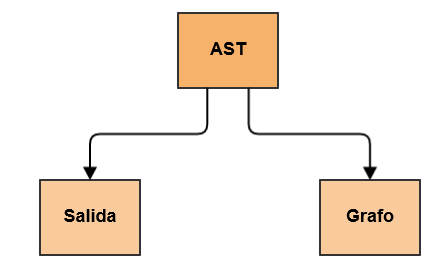
\includegraphics[scale=0.55]{imagenes/Compilacion_parte_1.png}
	\end{center}
	\caption{
		\label{fig:compilacion_part_1}
		Compilación parte 1
	}
\end{figure}

\subsection{Parte segunda: Cálculo del dominio} \label{solver:dom}
En esta parte se obtendrán los posibles valores iniciales que puede adoptar cada 
variable. Para esto es fundamental la noción de conjunto que se había establecido.
El cálculo del dominio se efectúa de la siguiente forma:
\begin{enumerate}
 \item {Para cada variable no instanciada, de tipo básico encontrada en el \textbf{AST} y
  que haya sido creada también en la estructura de salida, se crea un nodo en el 
  grafo. Las variables de tipo estructura no serán consideradas para esto, pues sólo son 
  referencias para las de tipo básico.}
 \item {Si la variable es de un tipo básico, entonces a su nodo en el grafo se le 
  añaden las restricciones propias.}
 \item {Luego de desplegar la estructura de salida esta misma se recorre en orden 
  inverso. Entonces las restricciones propias de las variables estructurales se 
  añaden a la variable referenciada.}
 \item {En este mismo recorrido inverso se añaden las restricciones no propias 
  como arcos del grafo.}
 \item {En este punto cada variable cuenta con una lista de todas las restricciones 
  propias a si mismas. Luego, para cada uno de los nodos en el grafo se crea un hilo 
  para que se encargue de el cálculo de su dominio.}
 \item {El hilo, cuyo funcionamiento será explicado en breve deberá recibir  
  un archivo con las restricciones.}
\end{enumerate}

En resumen de lo que se estudia en esta etapa es lo que se muestra en la figura
\ref{fig:compilacion_part_2}.

\begin{figure}[h]
	\begin{center}
		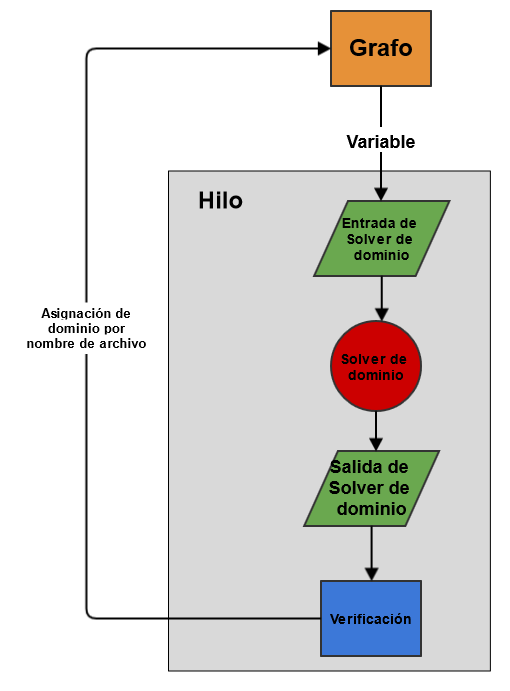
\includegraphics[scale=0.55]{imagenes/Compilacion_parte_2.png}
	\end{center}
	\caption{
		\label{fig:compilacion_part_2}
		Compilación parte 2
	}
\end{figure}

\subsubsection{Hilo para el cálculo de dominio}
Para cada variable se creará un hilo con el que se delimitará su dominio. Estos
hilos funcionarán de la siguiente forma:

\begin{itemize}
 \item {El hilo escribirá en un archivo identificado con un nombre clave para la 
  variable, todas las restricciones afines a la misma, estructuradas de forma que 
  el programa solucionador de dominio escrito en \emph{Prolog} pueda interpretarlo como un 
  predicado.}
 \item {Luego de escrito el archivo el hilo, espera a que el programa en \emph{Prolog} 
  al cual se le llamará a partir de ahora ``Solver de dominio'' o ``Solucionador de 
  dominios'' (sección \ref{solver_dom}) termine su ejecución.}
 \item {El \emph{solver} de dominio habrá escrito un archivo con el resultado obtenido.
  Ahora el hilo deberá abrirlo y revisar si hubo un error. Si lo hubo, el hilo se 
  encargará de la interrupción del programa, de lo contrario añadirá el nombre 
  del archivo a la información contenida en los nodos.}
 \item {El hilo termina su ejecución.}
\end{itemize}

A partir de este punto el programa esperará a que todos los hilos terminen su 
ejecución. Con lo que todos los dominios estarán ya calculados.

\subsubsection{\textit{Solver} de dominio o solucionador de dominio}
\label{solver_dom}
Este es un programa escrito en el lenguaje de programación \emph{Prolog} cuya función es 
utilizar \emph{backtracking} sobre los valores comprendidos en el rango de la variable, 
para conseguir todos los valores posibles que cumplan con todas las restricciones. 
La especificación del funcionamiento de este programa y sobre el uso de \emph{Prolog} 
serán tratadas en otro punto.

\subsection{Parte tercera: Cálculo de rangos}\label{solver:cal_rangos}
La dinámica para el cálculo de rangos es similar a la del cálculo de dominios, 
solo que adicionalmente se deben definir y separar los sistemas de variables 
antes de resolverse. Esto se hace de la siguiente forma:

\begin{enumerate}
 \item {El primer paso es aplicar el algoritmo de Roy Warshall \cite{CLR90} al 
  grafo para hallar la clausura transitiva de los nodos y así poder separarlos 
  por grupos. Estos grupos definen cuales son los sistemas de variables.}
 \item {Si existe algún grupo con una sola variable entonces se considerará que 
  este sistema está resuelto y se modificará el nombre del archivo de dominio 
  asociado a esta para ser utilizado como rango del sistema.}
 \item {Para cada sistema se crea un hilo que actuará de forma idéntica a los que 
  trabajan los dominios, con la excepción de que estos transcribirán las 
  restricciones de forma diferente y llamarán a otro programa en \emph{Prolog} distinto 
  para que resuelva las rangos. Este programa será llamado ``Solver de rangos'' 
  o ``Solucionador de rangos'' (sección \ref{sol_rangos}).}
 \item {Al recibir respuesta por parte del \emph{Solver} el hilo revisa si el archivo 
  contiene algún error o si el rango es vació. Si todo es correcto escribe la 
  dirección del archivo en la representación del sistema.}
\end{enumerate}

Luego de este punto el grafo es innecesario y puede ser olvidado o destruido. De la misma forma ,
no hace falta almacenar los archivos de dominio. En la sección referente a 
la optimización se hablará más de esto. Un resumen de lo que se genera en esta 
etapa es lo que se muestra en la figura \ref{fig:compilacion_part_3}.

\subsubsection{Solver de rangos o Solucionador de rangos}
\label{sol_rangos}
Este programa actúa de forma similar al \emph{Solver} de dominios, su diferencia con 
este reside en que este primero toma como entrada los archivos correspondientes a 
la variables del sistema y adicionalmente recibe un archivo escrito por el hilo 
quien lo llamó, que contiene la especificación de las restricciones que tiene el 
sistema. Por último este programa retorna la dirección del archivo que escribe 
con la información de los posibles rangos del sistema.

\begin{figure}[h]
	\begin{center}
		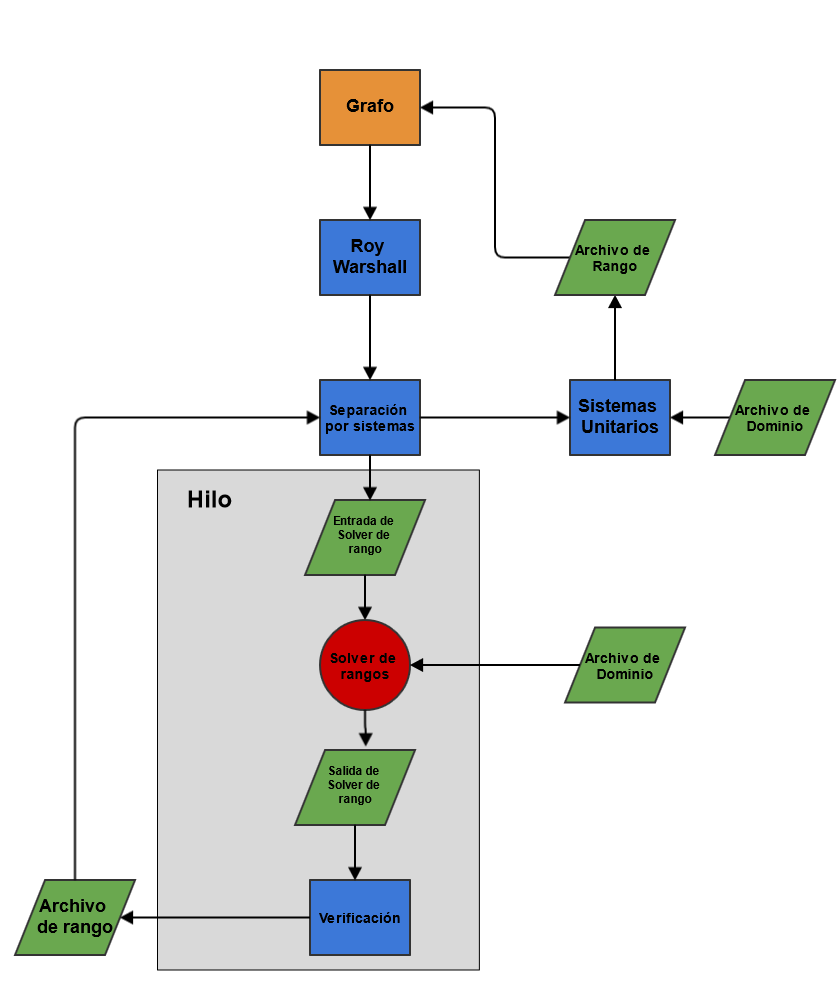
\includegraphics[scale=0.4]{imagenes/Compilacion_parte_3.png}
	\end{center}
	\caption{
		\label{fig:compilacion_part_3}
		Compilación parte 3
	}
\end{figure}

\subsection{Parte cuarta: multiplicación de rangos}
Una vez conseguidos los rangos para cada sistema solo falta unir estos resultados 
con los de los demás sistemas para conseguir soluciones finales.
Esta parte del compilador es relativamente simple puesto a que sólo hay que hacer 
la multiplicación de los vectores de rango. Para esta operación se debe decidir 
de forma aleatoria una solución de cada sistema y unirlos. Una forma gráfica de 
verlo es tal y como luce en la figura \ref{fig:compilacion_part_4}.

A partir de este punto no hace falta almacenar los archivos de rangos.

\begin{figure}[h]
	\begin{center}
		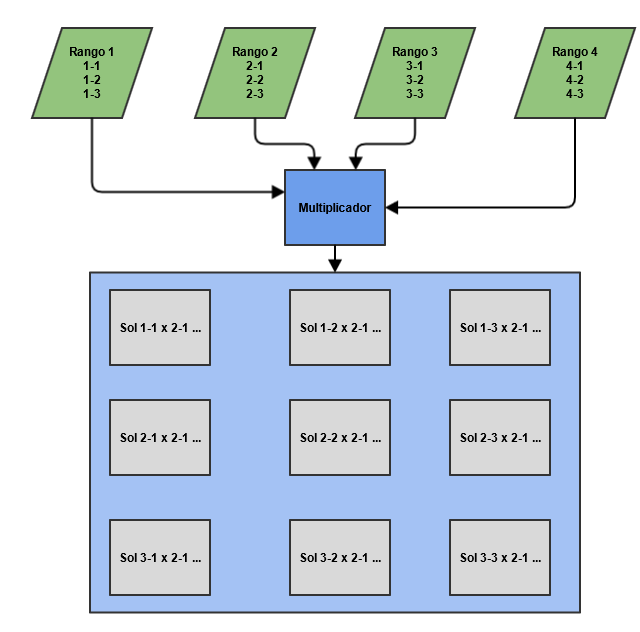
\includegraphics[scale=0.5]{imagenes/Compilacion_parte_4.png}
	\end{center}
	\caption{
		\label{fig:compilacion_part_4}
		Compilación parte 4
	}
\end{figure}

\subsection{Parte quinta: Instanciación de valores}
Una vez obtenidas las soluciones finales, resta únicamente instanciar la 
estructura de salida con los valores de las variables de cada solución y reducir
la salida de las soluciones solicitadas por el usuario. Esta salida se realiza en un 
formato genérico en \emph{JSON} para que pueda ser interpretado y utilizado por 
otro programa tal y como se muestra en la figura \ref{fig:compilacion_part_5}.

\begin{figure}[h]
	\begin{center}
		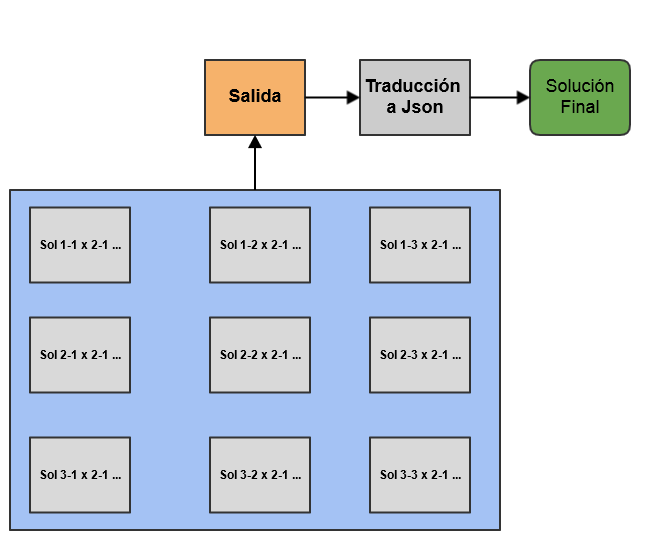
\includegraphics[scale=0.5]{imagenes/Compilacion_parte_5.png}
	\end{center}
	\caption{
		\label{fig:compilacion_part_5}
		Compilación parte 5
	}
\end{figure}
